\documentclass[11pt, a4paper]{article}
%\usepackage{proj1}
\usepackage{natbib}
\usepackage{fancyhdr}  
\usepackage{subcaption}
\usepackage{caption}
\usepackage{graphicx}
\linespread{1.25} 
\setlength{\parindent}{0cm}
\graphicspath{{Images/}}
\usepackage{hyperref}
\usepackage{amsmath}
\usepackage{amsfonts}
\usepackage{amssymb}
\usepackage{amsthm}
\usepackage{mathtools}
\usepackage{commath}

%\usepackage[sc,osf]{mathpazo}
\usepackage{subcaption}
\usepackage[a4paper, top=1in, left=1.0in, right=1.0in, bottom=1in, includehead, includefoot]{geometry} %Usually have top as 1in

\usepackage{listings}
\usepackage{color} %red, green, blue, yellow, cyan, magenta, black, white
\definecolor{mygreen}{RGB}{28,172,0} % color values Red, Green, Blue
\definecolor{mylilas}{RGB}{170,55,241}


\hypersetup{colorlinks,linkcolor={black},citecolor={blue},urlcolor={black}}
\usepackage{color}
\urlstyle{same}


\theoremstyle{definition}
\newtheorem{definition}{Definition}[section]

\title{Exact Solutions for the Full Problem \\with Force Control and with Flow Control}
\date{}
\newcommand{\Sta}{\rho}
\newcommand{\Adj}{p}
\newcommand{\Con}{u}

\pagenumbering{gobble}
\begin{document}
\lstset{language=Matlab,%
	%basicstyle=\color{red},
	breaklines=true,%
	morekeywords={matlab2tikz},
	keywordstyle=\color{blue},%
	morekeywords=[2]{1}, keywordstyle=[2]{\color{black}},
	identifierstyle=\color{black},%
	stringstyle=\color{mylilas},
	commentstyle=\color{mygreen},%
	showstringspaces=false,%without this there will be a symbol in the places where there is a space
	numbers=left,%
	numberstyle={\tiny \color{black}},% size of the numbers
	numbersep=9pt, % this defines how far the numbers are from the text
	emph=[1]{for,end,break},emphstyle=[1]\color{blue}, %some words to emphasise
	%emph=[2]{word1,word2}, emphstyle=[2]{style},    
    basicstyle=\footnotesize\ttfamily,
}
\section*{Additional Examples}

\section{One Dimensional non-symmetric gaussian $\hat \rho$}

We choose $\rho_0 = 0.5$ and
\begin{align*}
\hat \rho = 0.5(1-t)  + t\frac{1}{0.5604}e^{-10((y+0.2)^2)}.
\end{align*}
The prefactor $\frac{1}{0.5604}$ ensures that the mass of $\hat \rho$ is one at all times. Choosing $n = 61$, $N = 60$, ODE Tols $ = 10^{-8}$, Optimality Tols $= 10^{-4}$.
For $\beta = 10^{-3}$ and $\gamma = -1$, $J_{FW} = 0.1084$ and $J_{Opt} = 0.0055$, see \ref{FigExG1}.
For $\beta = 10^{-3}$ and $\gamma = 1$, $J_{FW} = $ and $J_{Opt} = $, see \ref{FigExG2}. Other choices of $\beta$ and $\gamma$ behave as expected.
\begin{figure}[h]
	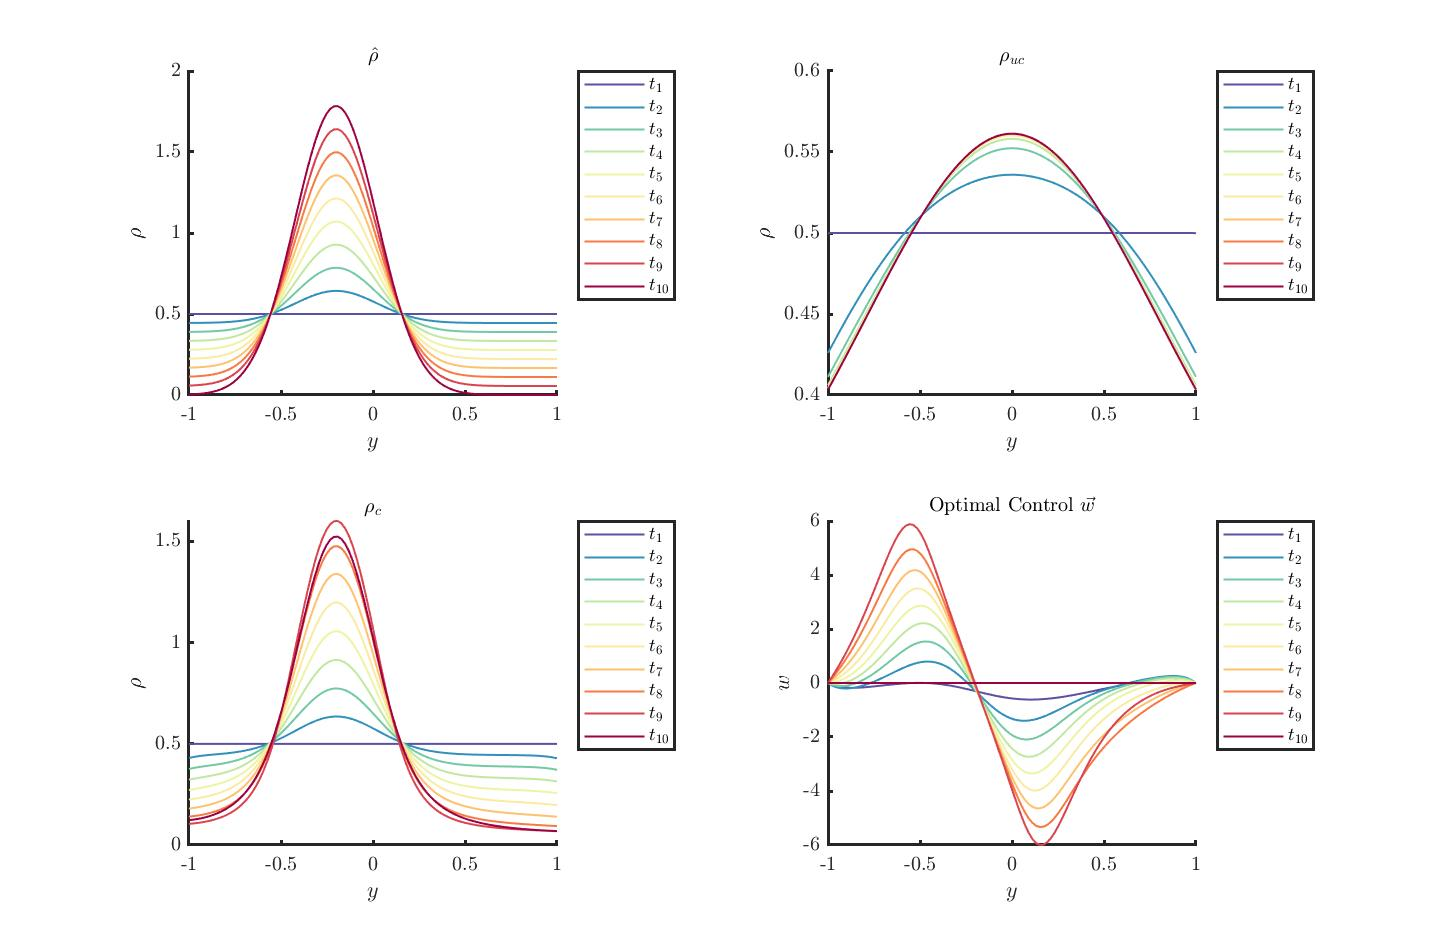
\includegraphics[scale=0.3]{ExG1.jpg}
	\caption{1D Example with $\beta = 10^{-3}$, $\gamma = -1$}
	\label{FigExG1}
\end{figure}
\begin{figure}[h]
	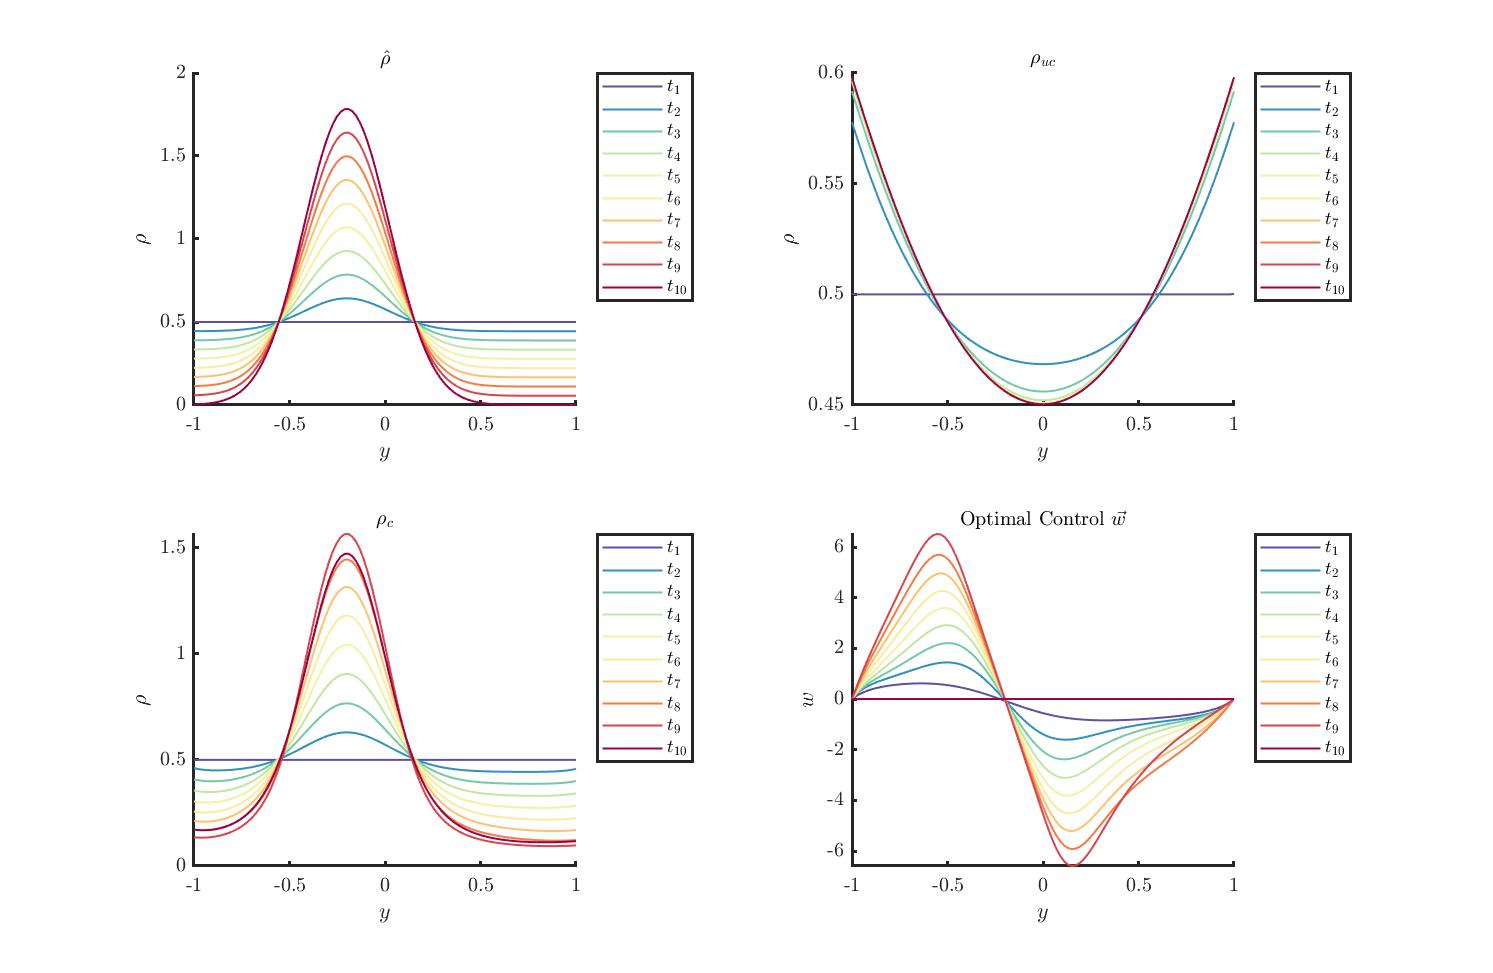
\includegraphics[scale=0.3]{ExG2.jpg}
	\caption{1D Example with $\beta = 10^{-3}$, $\gamma = 1$}
	\label{FigExG2}
\end{figure}
\section{Two Dimensional, Example 1}
++ 2D seems to work now because I fixed mass conservation, which wasn't correct the last time I ran it. ++\\
We choose $\rho_0 = 0.25$ and
\begin{align*}
\hat \rho = 0.25(1-t) + t*\frac{1}{4}((\cos(\pi y_1)+1)(\cos(\pi y_2)+1)),  
\end{align*}
see \ref{rhoHat2d1}
\begin{figure}[h]
	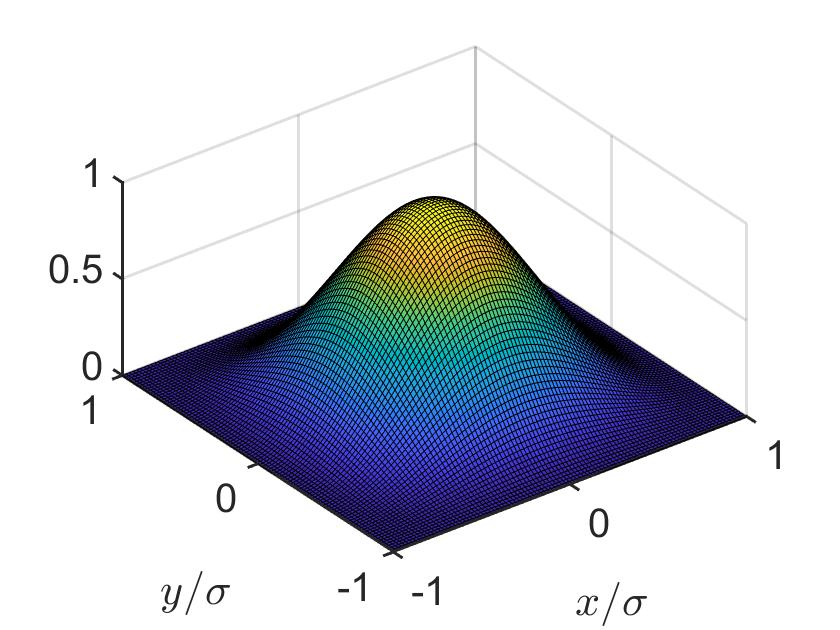
\includegraphics[scale=0.3]{rhoHat2D1.jpg}
	\caption{2D Example 1, $\hat \rho$ at $t=20$}
	\label{rhoHat2d1}
\end{figure}
We choose $n = 20$, $N_1,N_2 = 30$. Tolerances are $10^{-8}/10^{-4}$.
For $\beta = 10^{-3}$ and $\gamma = 1$, $J_{FW} = 0.0596$ and $J_{Opt} = 0.0170$, see \ref{Fig2D1}, \ref{Fig2D2}, \ref{Fig2D3}.
For $\beta = 10^{-3}$ and $\gamma = -1$, $J_{FW} = 0.0334$ and $J_{Opt} = 0.0020$, see \ref{Fig2D4}, \ref{Fig2D5}, \ref{Fig2D6}.
\begin{figure}[h]
	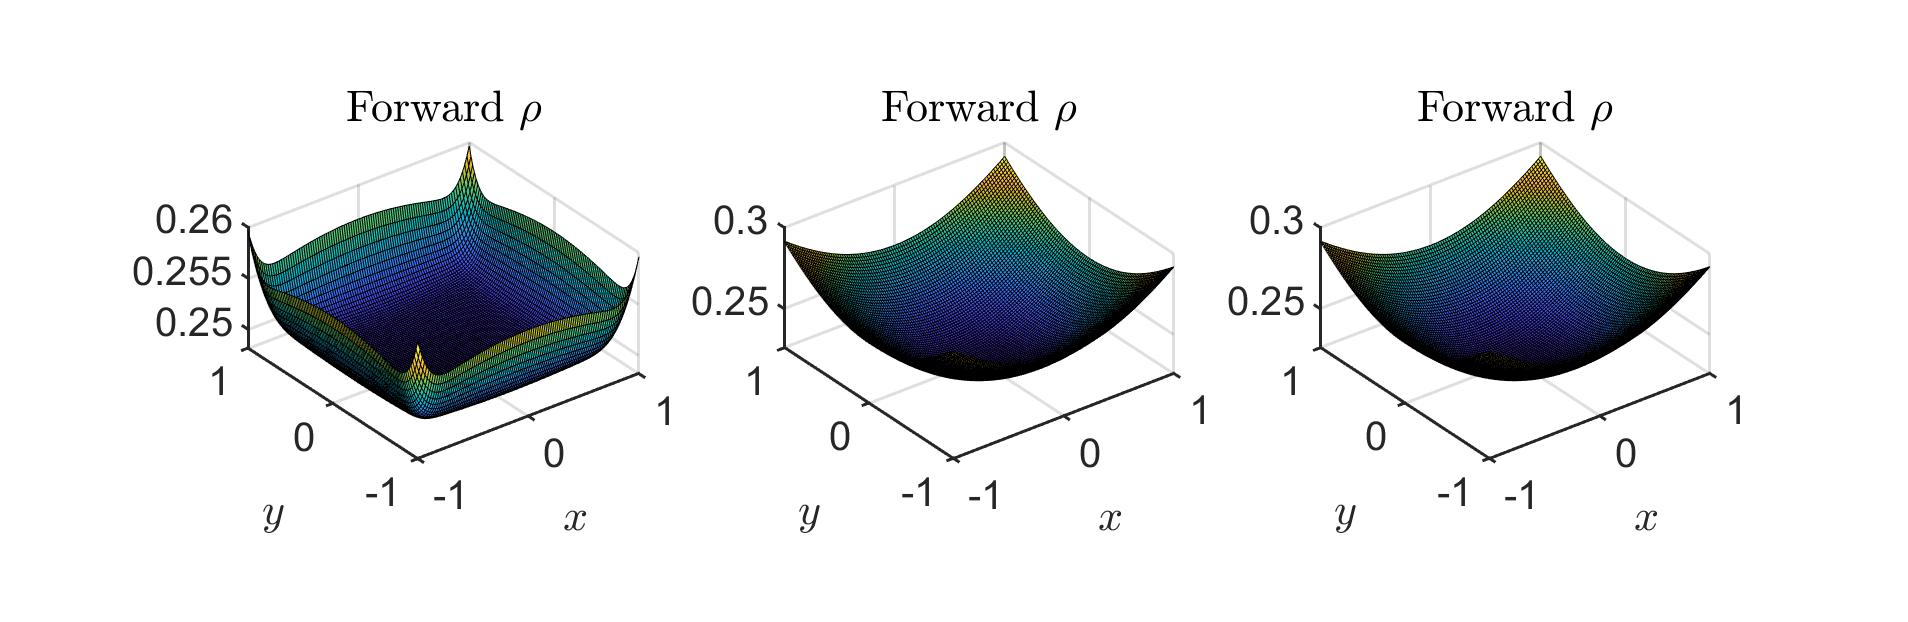
\includegraphics[scale=0.3]{FWrho2Dg1.jpg}
	\caption{2D Example 1, $\rho$ forward, $t= 2,10,20$, $\beta = 10^{-3}$, $\gamma = 1$}
	\label{Fig2D1}
\end{figure}
\begin{figure}[h]
	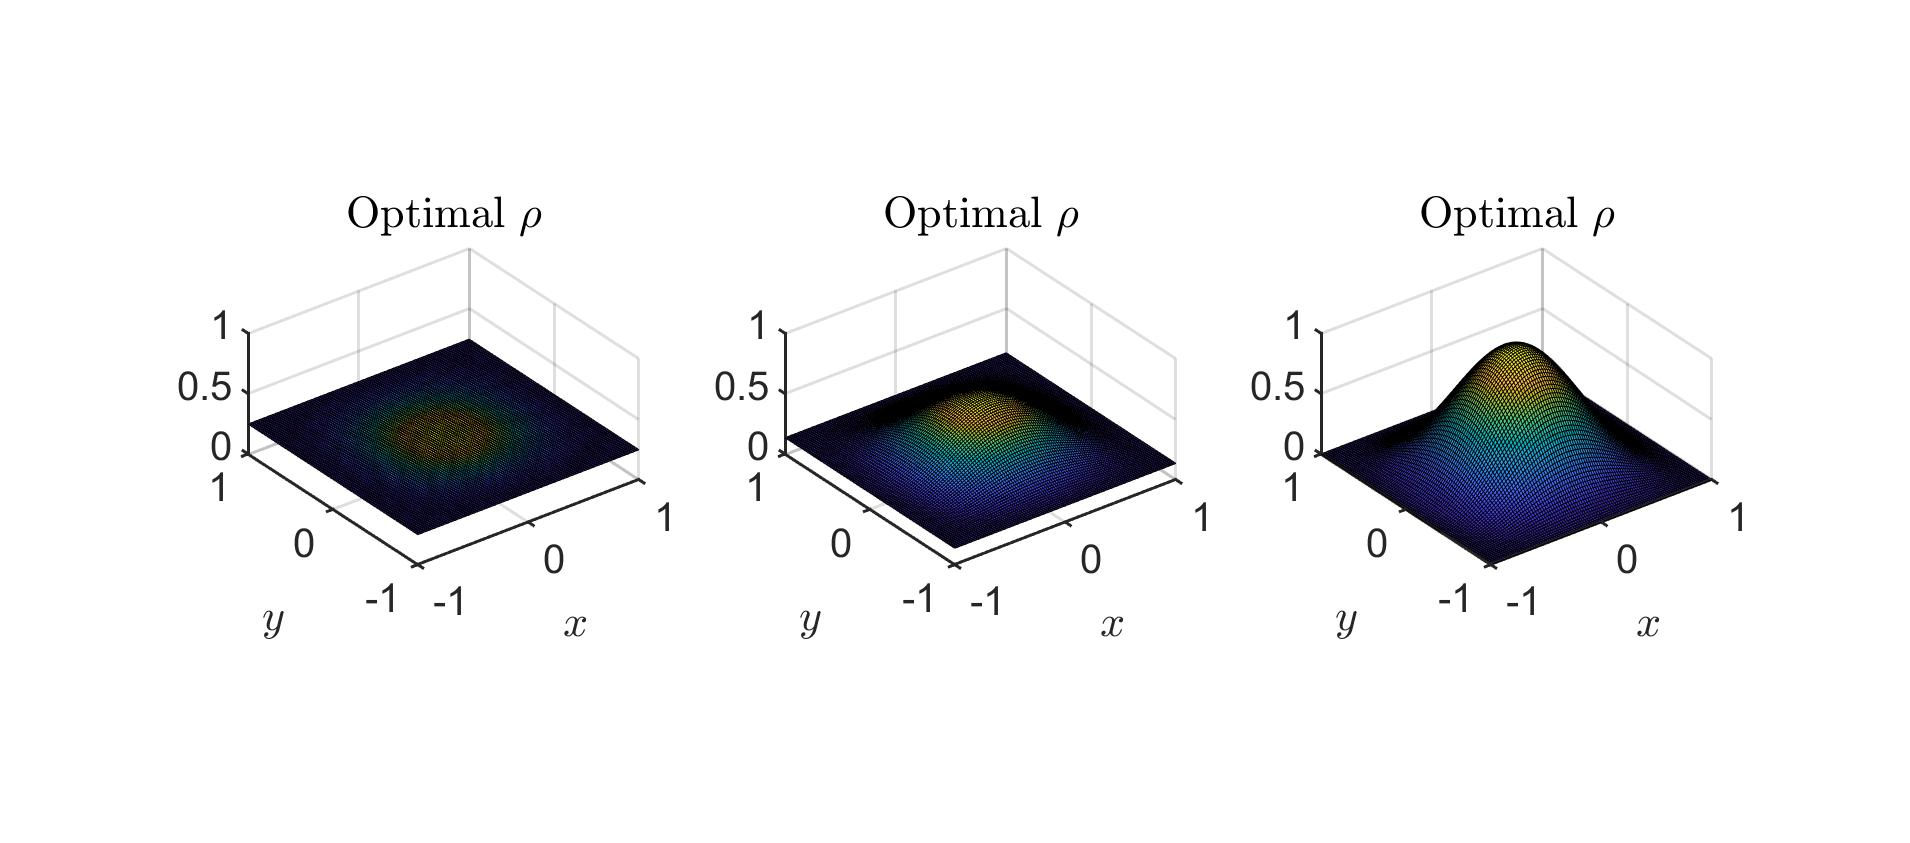
\includegraphics[scale=0.3]{Optrho2Dg1.jpg}
	\caption{2D Example 1, $\rho$ optimal, $t= 2,10,20$, $\beta = 10^{-3}$, $\gamma = 1$}
	\label{Fig2D2}
\end{figure}
\begin{figure}[h]
	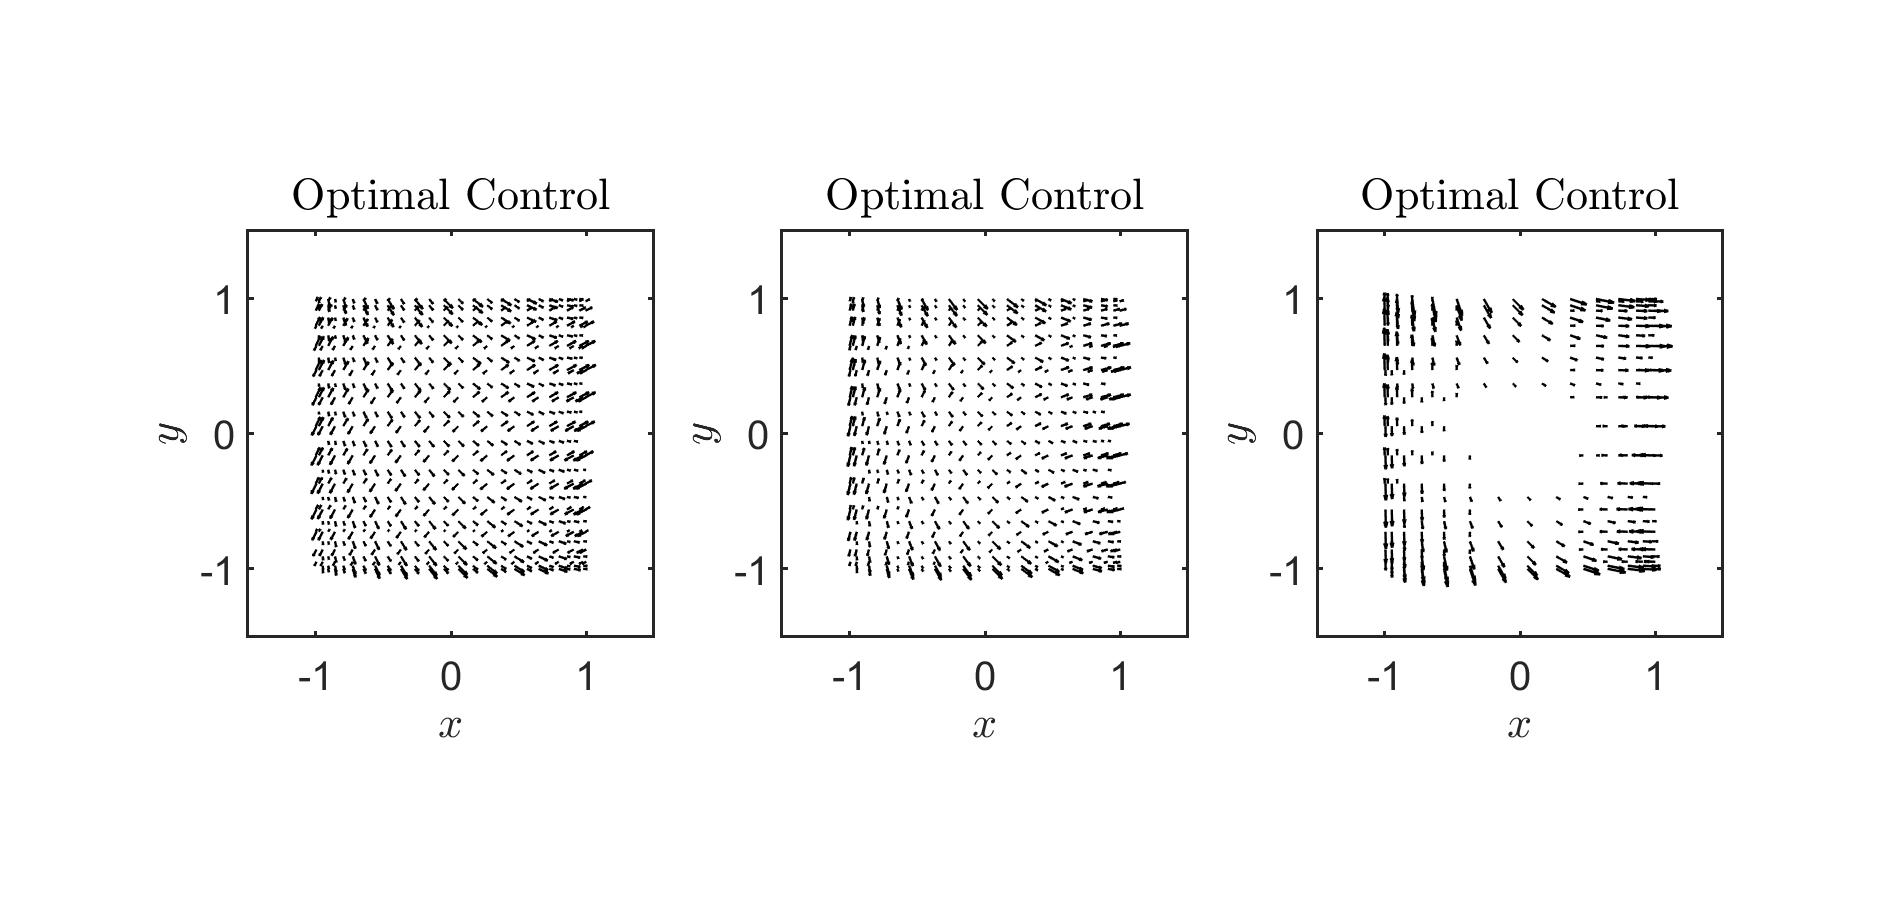
\includegraphics[scale=0.3]{OC2Dg1.jpg}
	\caption{2D Example 1, Optimal Control, $t= 2,10,19$, $\beta = 10^{-3}$, $\gamma = 1$}
	\label{Fig2D3}
\end{figure}

\begin{figure}[h]
	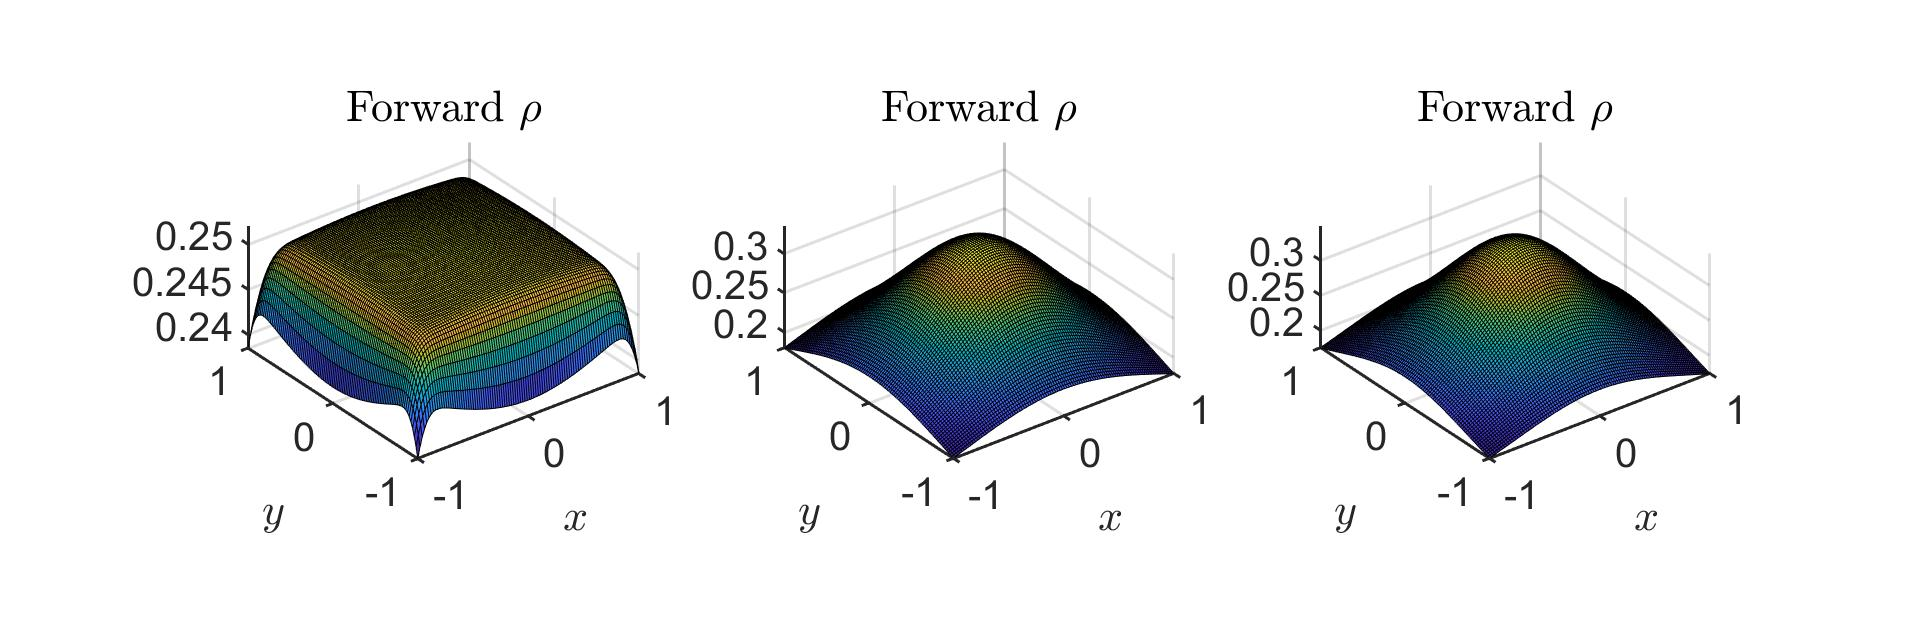
\includegraphics[scale=0.3]{FWrho2Dgn1.jpg}
	\caption{2D Example 1, $\rho$ forward, $t= 2,10,20$, $\beta = 10^{-3}$, $\gamma = -1$}
	\label{Fig2D4}
\end{figure}
\begin{figure}[h]
	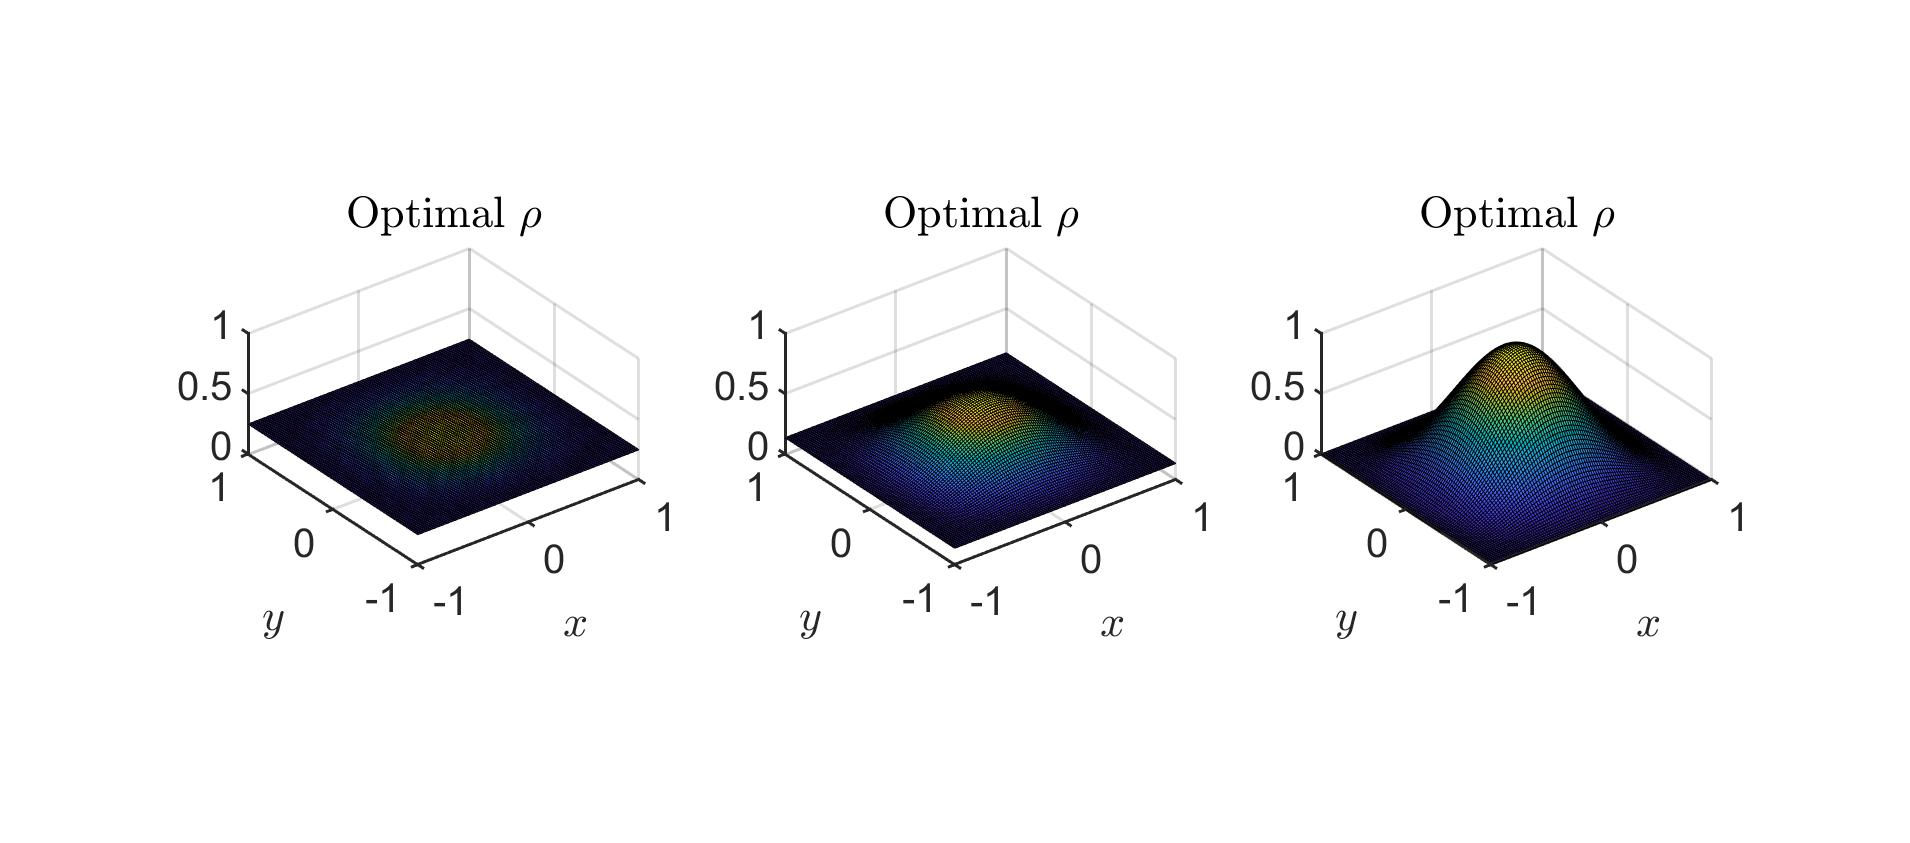
\includegraphics[scale=0.3]{Optrho2Dgn1.jpg}
	\caption{2D Example 1, $\rho$ optimal, $t= 2,10,20$, $\beta = 10^{-3}$, $\gamma = -1$}
	\label{Fig2D5}
\end{figure}
\begin{figure}[h]
	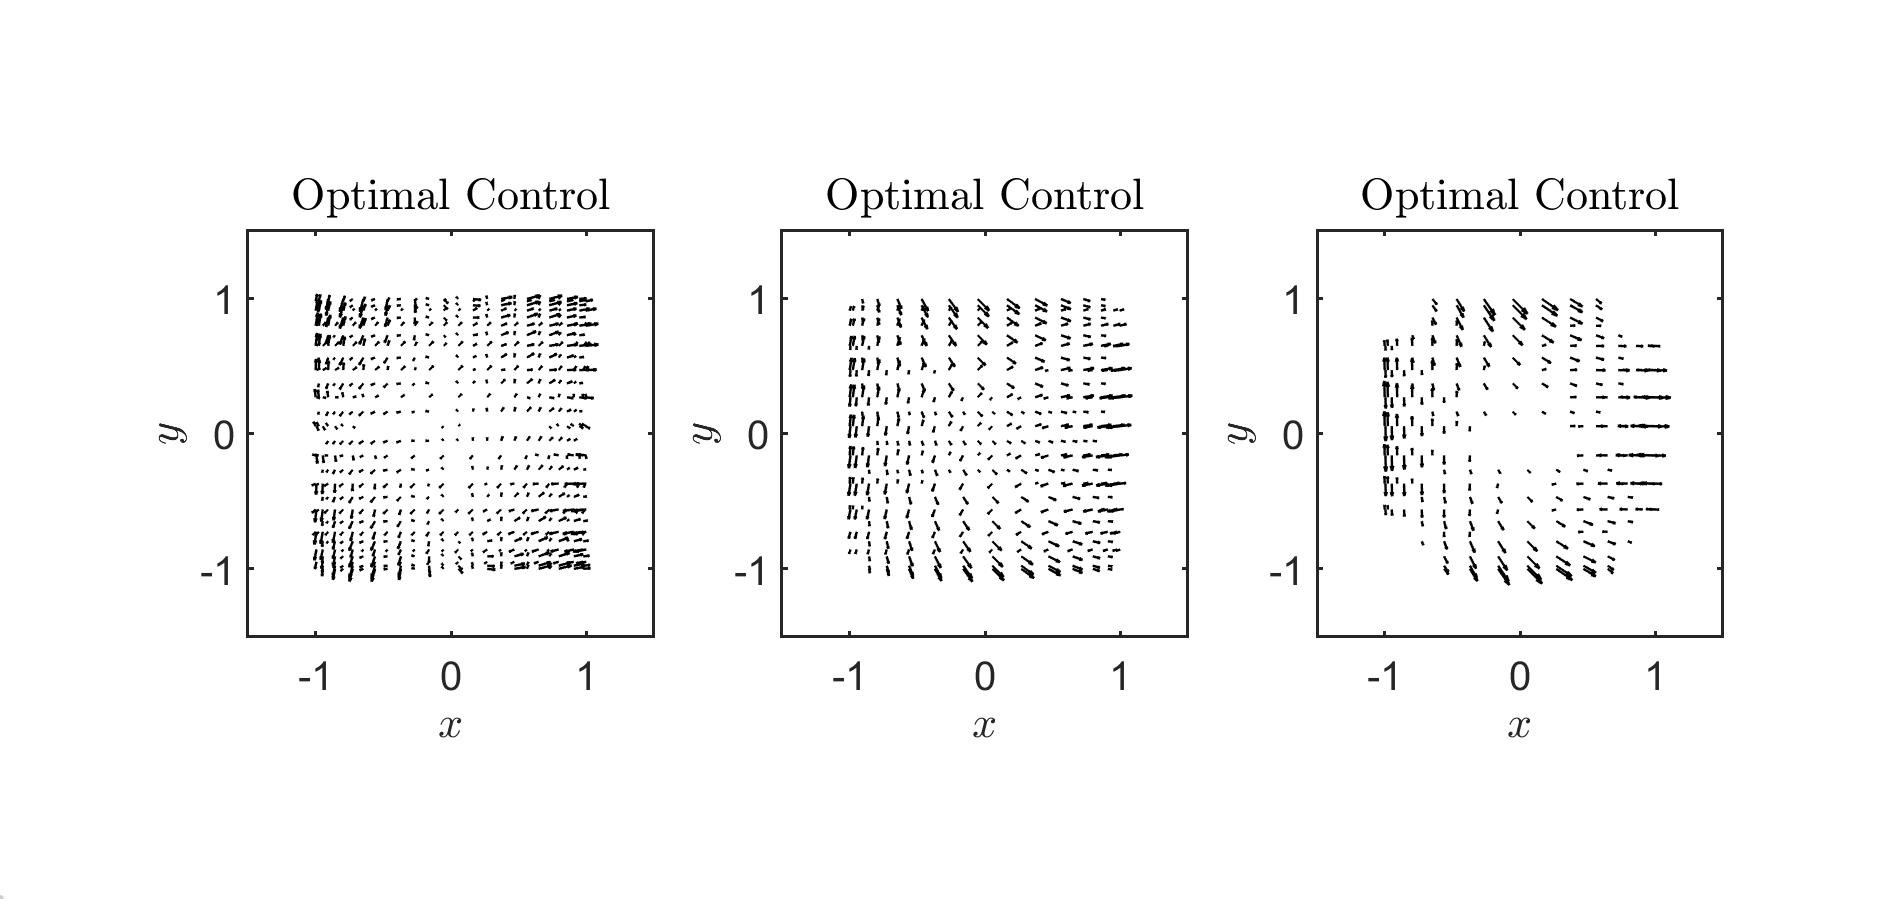
\includegraphics[scale=0.3]{OC2Dgn1.jpg}
	\caption{2D Example 1, Optimal Control, $t= 2,10,19$, $\beta = 10^{-3}$, $\gamma = -1$}
	\label{Fig2D6}
\end{figure}

\section{Two Dimensional, Example 2}

\section{Two Dimensional, Example 3}



\end{document}